\documentclass{article} % article doctype, possible font size range from 8pt to 20pt with not all being avaiable.
\title{\huge Willy The Robot Personal and Group Reflections}
\author{Jeroen van 't Hul\\S1139163  \and Thomas Zwaanswijk\\s1089273 \and Tom van den Noort\\s1101124}
\date{\parbox{\linewidth}{\centering%
	\today\endgraf\bigskip
	Supervisor \hspace*{3cm} Main Stakeholder \endgraf\medskip
	Mischa Mol \hspace*{3cm} Ilja Clabbers \endgraf\bigskip
	Windesheim Zwolle\endgraf}} 


% include packages
\usepackage{graphicx}
\usepackage{caption}
\usepackage{mathabx}
\usepackage{wrapfig}
\usepackage[margin=1.0in]{geometry} % sets page margin, 2.0in is default.
\usepackage{titlesec}
\usepackage{hyperref}
\usepackage[table,xcdraw]{xcolor}
\usepackage{float}
\usepackage[export]{adjustbox}
\usepackage{todonotes}
\usepackage{indentfirst}
\usepackage{blindtext}
\usepackage{scrextend}
\usepackage{apacite}
%\usepackage{siunitx}
%\usepackage{multirow}	% used for table multirow support
%\usepackage{longtable} % Allows tables to roll over into a new page.
\usepackage[nottoc,numbib]{tocbibind} % Adds bibliography / references to TOC and numbers that section.
\usepackage{array}
\usepackage{footnote}

% ----- custom commands ----- %
% Wrapper for paragraph command. Forces newline after paragraph title
\newcommand{\myparagraph}[1]{\paragraph{#1}\mbox{}\\} % Without \mbox{} all newlines will be ignored, making the first sentence appear on the same line as a paragraph title.
% monospace codeblock
\def\code#1{\texttt{#1}}
% changing the ToC depth in the document enviroment
\newcommand{\changelocaltocdepth}[1]{%
	\addtocontents{toc}{\protect\setcounter{tocdepth}{#1}}%
	\setcounter{tocdepth}{#1}%
}

\restylefloat{table}

\newcolumntype{L}[1]{>{\raggedright\let\newline\\\arraybackslash\hspace{0pt}}m{#1}}
\newcolumntype{C}[1]{>{\centering\let\newline\\\arraybackslash\hspace{0pt}}m{#1}}
\newcolumntype{R}[1]{>{\raggedleft\let\newline\\\arraybackslash\hspace{0pt}}m{#1}}

\makesavenoteenv{tabular}
\makesavenoteenv{table}

\setcounter{tocdepth}{2} % only part,chapters,sections, subsections appear in ToC

\addtokomafont{labelinglabel}{\sffamily}

\DeclareCaptionFormat{cancaption}{#1#2#3\par} % Normal format actually
\DeclareCaptionLabelFormat{cancaptionlabel}{#1}
\captionsetup[figure][number]{format=cancaption,labelformat=cancaptionlabel}
\graphicspath { {images/}{../images/} }

\begin{document}
\maketitle

\begin{figure}[H]
\centering
\includegraphics[width=12 cm]{WTRLogo.png}
\end{figure}
\thispagestyle{empty}
\newpage
\setcounter{page}{1}
\tableofcontents
\newpage

% Sections
\section{Introduction}
This research is meant to create an inventory of the current state of the movements WTR\ref{trm::WTR} is capable of performing.
In addition, this document contains a list of proposed improvements in order to increase the accuracy of the autonomous driving.
By creating a list of the range of movement WTR can perform and noting any defects or issues with those, it should become easier to create a proper list of improvements.
Several sections will deal with the sensors, how they benefit the robot and their mounting as well.
\newpage

%\section{Product}
\subsection{Current Status of Product}
In the current state, the driving capabilities of WTR have been improved considerably.
The functionality of WTR has been improved through inclusion of an IMU, rotary encoders and the sonar sensors.
While some of these were present at the start of the project, data was either being spoofed or simply not being utilized.

The IMU previously used, the MPU6050, for example was not actually used, and the data was being spoofed so that the robot would move more smoothly.
This has now been corrected, and the actual data received from the new MPU9250 is incorporated into the planning, as well as being more accurate than the old IMU.

The sonars, which previously were not used, are now utilized as well.
Several additional sensors are now located at the back of WTR, so that it can also detect obstacles behind it, so that even during reversing it can be safe.

\subsection{What Could Be Added?}
There are some features that could be implemented in order to increase the safety features of WTR, which are all documented in the separate advice document.
As such, it will not be expanded upon in this document.

\subsection{Schematic Overview}
Figure \ref{fig::schemView} shows the new situation of WTR.
More detailed explanations of every section can be found in the respective documents dealing with those sections.
\begin{figure}[H]
\centering
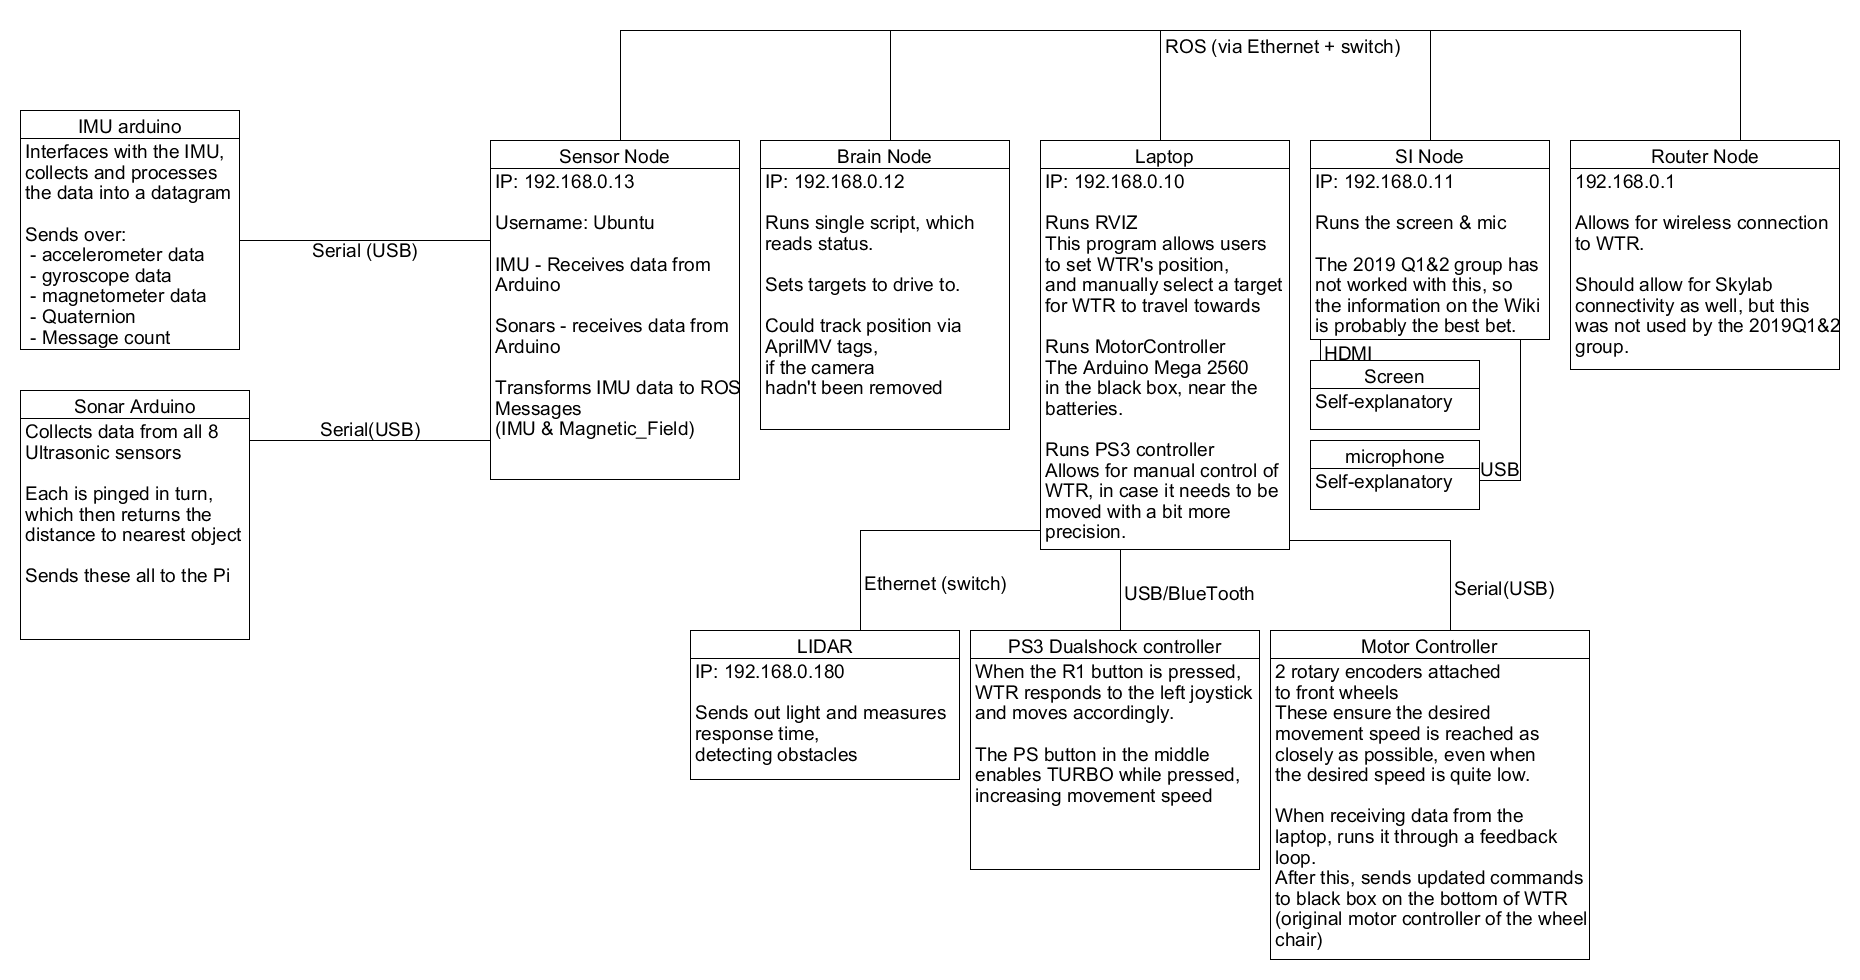
\includegraphics[width=15cm]{rosOverview.png}
\caption{An overview of the separate parts of WTR}
\label{fig::schemView}
\end{figure}

The sensor node communicates with the IMU and the sonar HC-SR04 sensors through arduinos over a serial communication protocol.
This allows easy changes to be made to either section without having to stop both at once, since the node will simply not do anything if it does not receive any messages.

The motor controller is an Arduino Mega 2560, which is connected to the laptop through a USB cable and uses a serial communication protocol as well to translate the commands from RVIZ to a format the P\&G \ref{trm::PGE} can understand and execute.
The feedback loop ensures that it can perform accurately at low velocity as well, rather than blindly sending a speed to it and assuming it is accurate enough to do so.

\newpage

%\section{Process}
This section details how the project was run, what methodology was used and how the quality of the separate parts of WTR were ensured.
At the end, there is also a short reflection about the processes as they were used during the project and what was learned from using them.

\subsection{Intial Intention}
\subsubsection{Methodology}
The chosen methodology for this project was SCRUM, since it is a methodology most of the group is familiar and comfortable with.
Another advantage that SCRUM offered for this project is that the scope can be flexible, since the exact goal of the project was not clear at the start.
Some parts of SCRUM were discarded, such as the daily meeting with the product owner, since the product owner would not have had time for that.

The sprints were set to be two weeks long, allowing for a total of 8 sprints.
This allowed the group enough time to focus in-depth on any single issue, without causing feature-creep [\ref{trm::FC}] in a sprint.
At the end of each sprint a sprint review was held with the product owner.
During this review, a small retrospective was also held to discuss sticking points and good performance.

\subsubsection{Weekly activities}
Every week, a meeting was held with either the product owner or the coach.
This turned out to be the same person, which was cause for apprehension at the beginning.
This fear turned out to be ungrounded, as Mischa Mol kept the two roles separate admirably.

\subsubsection{Process Overview}
Trello was chosen as a digital Scrum board.
While it would have been possible to organize a physical board, the environmental impact of a digital board is lower, and it is easier to pass on to new groups so that they can create an inventory of possible left-over tasks.
The board can be found \href{https://trello.com/willytherobot/home}{here}.
Several boards were created, though not all of them used.
The main bulk of the content is located in Project Tasks, with additional information found in the other board, TODO.

\subsubsection{Quality Management}
Several choices were made to ensure a consistent quality level.
First of all, all documents and code have been written in English, so that any international students can also work on this project without having to rely on Google translate or such programs.
Secondly, a DOD [\ref{trm::DOD}] was made, which can be found in the project plan.
Some examples from the DOD are:
\begin{itemize}
\item Relevant documentation must be up to date, and checked by at least 1 reviewer
\item All code is uploaded to their proper branch, and checked by at least 1 reviewer
\item If changes have been made to the configuration or other parts of the code, update relevant sections
\end{itemize}
Additionally, in order to keep up to date with documentation and integrate with the pre-existing repositories, Git was used to ensure proper version control.
Every bit of code had to be reviewed by at least 1 person who didn't write the code.
This process was not necessarily enforced through pull request limitations, but rather through asking other members of the team to help out or check to see if the program functioned as intended.

\subsection{Correct Decisions?}
It is impossible to consider every aspect and consequence of a decision and still get work done, so sometimes a choice or decision has unintended effects. 
For example, despite the Git being organised into branches, due to a misunderstanding this was ignored a few times causing documentation to be in the wrong branch.
Does having to fix this and waste time on what is essentially an administrative error make using Git a mistake?

Git was useful, despite having caused the issues mentioned before.
The ability to easily keep code and documentation organized and up to date is worth the hassle it caused.
The reverting features of Git are also great, since several times they prevented having to redo entire sections due to over-eager deleting of documents.

Choosing SCRUM could be considered a mistake, as the nature of the project, which already has an existing base and product, means that the flexibility of SCRUM is negated by the inflexibility of the product.
However, since the group already has experience in SCRUM, this made the planning easier as tasks are clearly split up into single tasks.



\newpage

%\section{Security}
There are essentially two aspects to the security of WTR.
The first is the risk a malicious third party could pose to WTR if they wanted to abuse it.
The second is the risk WTR poses to the world around it.

\subsection{Vulnerabilities}
Ideally, WTR should be an air-gapped robot, with no possibility of wireless access, since it is going to be driving around at public events.
If WTR is broadcasting a network, then it would be possible to enter that and start commanding WTR to drive into people, for example.
Since this is unfortunately not possible as several social interaction features require an internet connection to some degree.

The likelihood of someone wanting to abuse WTR is quite small.
It has no connection to the network at the time of writing, and does not track any personal data.
There is essentially nothing of value to be gained by hacking WTR, so if it was done, it would most likely happen for the sake of a joke or prestige.
It would not exactly be difficult to hack either, due to the standardized nature of ROS.
ROS has set formats for every message, so a spoofed message to the \code{cmd\_vel} topic could cause WTR to over-accelerate, or drive straight into a wall.

Another vulnerability is that if someone has physical access to the switch, they could start spoofing messages and causing WTR to either crash or start behaving anomalously.
In order to prevent this, a small cover or physical protection could be used, such as a plexiglass cover that allows the internals of WTR to remain visible while preventing undesired physical access.

It would be advisable, however, to ensure that WTR gets an upgrade to its passwords.
Unfortunately, this group did not have the time to do this, but many of the passwords are vulnerable to botnets or other malicious attacks that exploit default passwords.
Many passwords are very weak, and could do with some updates.

\subsection{Danger to Others}
At the moment, WTR is a lot less dangerous to the world around it than it was at the start of the project.
Previously, it had several sharp edges that ended up costing a member of the team a pair of jeans, so the issue had to be taken care of.

Since then, it has had covers placed over all sharp edges that could hit someone while WTR is moving.
There are still some sharp bits, but due to a lack of angle grinder this group was unable to fix this.

The batteries are still only kept in place due to their weight, so a sudden stop due to a collision or abrupt stop signal could shift the batteries, potentially snapping cables or such.
As is noted in the advice document, this needs updating.
Another point mentioned is the exposed parts, which while not life-threatening as the batteries only run at 24 volt, are still not exactly good to have exposed.
Again, refer to the advice document for the group opinion on how to solve these issues.

\newpage

\section{Reflections}

\subsection{Jeroen van 't Hul}

\subsubsection{Introduction}
As being a mechatronics student from Saxion following the Minor Future Technology I tried to apply my knowledge of mechatronics into our project, and share it with my team members. 
My role in the project group is being the project leader, this mainly includes keeping in contact with various stakeholders and other members of Future Technology. 
As for the project itself the role was less visible as my team members kept initiative very well. 
In this reflection I will discuss the results I've achieved and make a conclusion afterwards.


\subsubsection{Results}
Throughout the project I've worked on various beneficial parts. 

Mechanically I've improved the wheel mounting/suspension of the robot, designed and realised various mountings for sonar sensors, the lidar sensor, rotary encoders, IMU and Arduino's. My design knowledge also inspired Thomas to learn 3D modelling and 3D printing.

Electrically I designed a wire harness for the rotary encoders and for the sonar sensors. 
The harness is compact and provided with connectors which is a huge improvement over the previous sonar setup.

On the programming side, the motor controller code is drastically changed to read out rotary encoders, include two PID loops and one controller. 
In order to check the control loop and tune the PID parameters I designed a viewer with charts, which also turned out to be very useful in understanding the drive and turn messages from ROS, and tuning accordingly.
For the 9 axis IMU I also designed a 3D viewer to get a better understanding on the output of the sensors.
The code for the sonar sensors on the Arduino and the Pi was drastically changed. Now RVIZ shows the sonar data individually on the map.
I also spent a lot of time in tuning parameters for the AMCL. This unfortunately did not gave the appropriate results. 

Documentation was written and updated on various parts. 
I updated the wiki on the parts I've worked on. 
New parts were written in analysis-improvements, tech design and hardware design on the parts I've worked on. 
I tried to support the text by means of self-explanatory flow charts, tables and wiring diagrams, which can be a great way in understanding more complex parts of WTR. 

\subsubsection{Conclusion}
Being a multidisciplined project I've learned a lot during this project, also from my other team members.
From them I got a basic understanding of GitHub, learned to document with \LaTeX, got insight into ROS and Linux. 
Personal 3D printing and CAD drawing skills have improved. 
I also had to heavily apply knowledge from control engineering to be able to get the robot to drive smoothly with the control loop.

On the other hand I failed to fix the drift issue in the AMCL on which I spent too much time, this was a bit demotivating and this motivation reflects on the team. This is something to look out for personally. 
Also the task dividing was very specific, it will help to get faster to good and complex solutions but it prevents us from being able to take over all possible tasks from each other. 
For example it would be better if I had spend more time in understanding ROS and RVIZ to be able to contribute on that part. 
Now this part was solely handled by Tom.

\newpage

\subsection{Tom van den Noort}
At first, I was excited to start on this project considering the mixture between hardware and software. 
This excitement had dwindled after our first in-depth examination of WTR. 
A lot of improvements needed to be done and as such; we were slightly worried if we could achieve most of these, but we've exceeded our expectations.
Integrating, improving, swapping new software plugins into ROS. We've gone through a few options to discover how simple our additions were, but we were met with challenges throughout.

\subsubsection{What went well?}
The start had not been the greatest, with the existing documentation having some incomplete parts, we learned how to start up some software plugins i.e. RViz, but how do you actually use and configure them?
Despite this, I've personally had no difficulty with absorbing the required information from the ROS wiki and other manuals to know the ins and outs of ROS itself. 
A notable achievement had been my investigation into the local planner; that would design paths for the robot to follow.
I've found that the one in the start of the project would just plan \textit{one} path and no other, which meant that if that path were to be blocked; the robot wouldn't know how to get past it, and spin in place, hoping the obstacle would be gone.
On the wiki page of this local planner I had found references to other planners, and after asking myself: ``What if I used one of those alternatives?'' I've looked at how to implement one of those, and I was surprised at how simple the swap was. 
More importantly; I was amazed by the great improvement of the new Timed Elastic Band Local Planner: It would dynamically recalculate the fastest path if an obstacle was thrown in front of it!

\subsubsection{What didn't go well?}
There was a downside to fiddling around with the software plugins and configuration files.
I did keep track of either what values I would change nor the original state of those, meaning that if the plugin were to behave erratically or cease function all together; I had nothing to turn back to if it worked well before my meddling. 
Although we did recover from such situations whenever they occurred, I did wish I would have made a back-up of the files in question before changing them.
Even if that will imply that there'd be an incremental back up every few minutes.
Similarly, whenever there would be an issue we cannot resolve by ourselves, we lost the motivation to continue and wound up procrastinating. 
This happened with the (re)integration of the IMU sensor. 
We had already loathed the time wasted upon compiling the code and to discover that it would still function incorrectly made the stockpile even bigger, to the point we opted to take a break.
In the end, it took us around four or more weeks to get the IMU to function and integrated within ROS.

\subsubsection{What comes along for the ride?}
It was a delight to work with students from other directions than Software Engineering or Business IT \& Management. 
The knowledge we've shared had certainly helped us along the way with this project, including the usage of tools as \LaTeX, which Thomas has explained very well. 
Jeroen shared his mechanical designs and knowledge, notably of 3D printing and sensor diagnostics and was more than excited to do so.
The three of us joined forces in the project and have learned much about algorithms, maths, C++, Python and the publisher/subscriber model which ROS is based off of.
I myself have gotten interested in this model and might apply it in future projects.
3D Printing is exciting, with plenty of possibilities, if it so happens that I would get involved with a project for Internet of Things devices, the skills I've been taught would be of great help.
In terms of documentation, \LaTeX would save considerable time generating neatly designed reports without the instability of Microsoft Word templates.


\newpage

\subsection{Thomas Zwaanswijk}
This project has been a mixed bag, in my honest opinion.
Some parts went very well, such as integrating new data into ROS, or the accidental discoveries that made the project what it is today.
Naturally, it wouldn't be a mixed bag if there were only positives, so to provide the counterpoint the IMU had to be very difficult to get right.
I did end up learning a lot from this project, ranging from picking up where others left off, to complex mathematics I would never have thought I would use.

\subsubsection{What Went Well?}
Personally, I'm very happy with how the appearance of Willy has been improved.
It went from being a jumble of cables leading to hard-to-access Raspberry Pi's to something that resembles a decently organized machine.
Obviously, there is still room for improvement, but the simpler setup WTR has now really does allow for easier maintenance and upgrades.
Removing the very wasteful massive cables has been great to do, as well as placing every device in an accessible location to allow easy maintenance.

Another great point is that the 3D-printing adds to the concept of future technology very neatly.
A lot of the improvement in the visual aspect of WTR comes from the fact that the previous layers of tape have been replaced by neat boxes containing all the sensors and components of WTR.
I'm very happy with how some of those turned out, as at the beginning of WTR I did not have a lot of experience with 3D-modelling in Solidworks, but I learned a lot of neat new tricks throughout this project.

\subsubsection{What Went Less Well?}
But to the good must eventually come the bad, and in my case this is the IMU.
I must have spent at least a week trying to understand the mathematical principles behind quaternions, though that did pay off in the end.
Updating the code to work with the new MPU9250 was a nightmare.
Having to work on code made by people who think \code{TeaPotPacket[]} is a descriptive variable name is a painful process, to say the least.
Adding to this were the complexities that showed up when attempting to transmit floats on a serial communication system, which can only handle 8-bit integers.
Eventually I got through it all, but I did waste a lot of time, which is my biggest regret of the project.

I also ended up procrastinating a fair bit when code wouldn't work or I ran into issues I couldn't solve.
Personally, I find it very demoralizing to have worked on some code for several hours only to find it's essentially useless because a minor technicality prevents it from working.
I suppose this is also why it took me so long to get the IMU working.
I have a bad habit of putting off the hard tasks until last, so I can at least have the feeling of having done something by finishing up some easy tasks.
I did suppress this habit later on in the project, because I started feeling the pressure of the time limit approaching and I didn't have any choice but to get things done.

\subsubsection{Multi-Discipline Work}
It was also nice to work in a multi-disciplinary team, despite it also producing some unique challenges.
I had to push quite a lot to get the group to adopt the use of \LaTeX, but in the end I'm very glad that I did since it makes keeping documentation up to date a lot easier.
It was also nice to learn about some new ways of dealing with data from Jeroen, such as moving averages and feedback loops.
Having never worked with these before, I ended up learning a fair bit about how to implement those systems and what benefits they offer.
Another nice part of working in this team was that everybody had something to contribute.
Tom was great at working with ROS, RVIZ and Linux, which probably would have taken me half the project to get to grips with.
Jeroen, as I mentioned earlier, was great at working with the mechanical aspects, and his 3D-designs skills are top notch, which ended up teaching me a lot.
The downside of this would be that I ended up learning less about the new systems than I would have if I had to work on them myself.
But then again, if I'd had to do all this by myself, I would not even have gotten a third of the work done, so I'm quite happy with the end result.

\subsection{Group Reflection}
As a group, we are pleased by the product we have created.
WTR is now capable of much more refined movement than it was capable of at the start of the project.
We have yet to test it in a situation like would be present at Winnovation, but the testing done on T5 has already shown that the current WTR is capable of avoiding humans and obstacles that were not present during the initial planning phase.

That is not to say that this project was without any strife.
There were periods of lacking motivation, such as when the IMU would not work or the map kept drifting away from reality.
This was a trap we fell into more than once, which just goes to show how de-motivating parts of this project were.

On the other hand, the feeling of finally getting parts working together and slowly seeing WTR turn from a large mess of cables on wheels that crashed after driving 15cm into something that we can almost be proud of that drives autonomously is a very rewarding indeed.
At the end of the project when testing its navigation, we did not even feel the need to continually stand next to it hovering our hand over the emergency stop, as we did in the beginning.
We'd just sit at our desks and watch as Tom set goals through a VNC/Remote desktop solution.

There were a variety of tools used to achieve the product, such as:
\begin{itemize}
\item Github - Version Control
\item Catkin - Compilation of code on the Raspberry Pi's
\item C++ - although we did not use a standard IDE within the group, we all ended up programming a fair bit in C++ in order to work with received data on the Pi, or in order to control the Arduinos
\item Python - Many scripts were written in Python as the simplicity of them did not necessitate delicate control over data-types or such
\item ROS - The backbone of the product, which supports and links all of the existing parts together
\end{itemize}
Not all of these tools were exactly appreciated, such as ROS, which while useful as a standardized tool, also has some really obfuscated documentation at times.
Another issue with ROS was that we misunderstood the way it worked at the beginning, which caused us to waste a week or so investigating the wrong things, such as believing code to be in places it wasn't.

Catkin caused quite a headache at times as well.
The raspberry Pi does not have a lot of RAM \ref{trm::RAM}, so compiling on just that system is a challenge, especially since Catkin also performs a lot of additional tasks, such as tracking dependencies and building files.
This had us stumped for a few days, since we couldn't get our heads around cross-compiling.
Eventually, we ended up making a swap-drive, which allowed the raspberry pi to use that as RAM and compile nonetheless.

On the whole, however, this was a valuable learning experience.
Having to pick up the project from other students was a great learning experience, showing just how important proper documentation is and how much value that can add to other contributors to a project.
This is something that has to be learned from experience, rather than being taught in a lesson.

We're all quite happy with how tasks were divided, but it would have been good to involve each other slightly more in some of the more crucial bits of each separate part.
As it stands, none of us could explain every part of the project to a complete outsider.
This is something we ran into because we all focused on our specialised parts, which means that they got done quicker, but it did limit the spread of information a bit.

\newpage

\appendix % all sections after this are appendices
\section{Glossary}
\begin{itemize}
\item \label{trm::dms} Dead-man's switch - a button on a controlling unit which has to be held down in order to have the robot respond to inputs. This is generally done in order ensure a machine cannot perform any actions should the controller be dropped or receive inputs without proper supervision.
\item WTR - Willy The Robot.
\end{itemize}
% Bibliography:
%\newpage
%\bibliographystyle{apacite}
%\bibliography{references}


\end{document}
